\documentclass{article}
\usepackage[utf8]{inputenc}
\usepackage[margin=1in]{geometry}
\usepackage{graphicx}
\usepackage{float}

\author{Alon Krauthammer, Mark Kubiak, Chris Munoz, Eashan Samak}
\title{ECE C247 Final Project\\
Methods}

\begin{document}
\maketitle

\section{Detailed Results}
Table \ref{tab:acc} shows the validation accuracy and the test accuracy for each
model we evaluated. As mentioned in the formal report, we used 20\% of the
training set provided as validation set, and trained on the remaining 80\%.

The accuracy results for the SCNN model and the SCNN augmented with LSTM and
attention mechanism were the best results out of five runs with the same
training and validation split.
We did not run $k$-fold cross validation as this would have required more
compute power than what we had available. Additionally, the hyper-parameters
used were the result of a handful of runs; again, since compute power was
limited, an exhaustive grid search was not feasible. Therefore, we believe
there's still room for improvement on the performance of this model on the BCI
IV dataset 2a. 

In addition to the task of classification across all subjects, we trained our
shallow CNN for the task of subject-specific classification.
Figure \ref{fig:subj-acc} shows the average test accuracy for each subject, with
and without input data standardization and cropping.

\begin{figure}[ht]
    \centering
    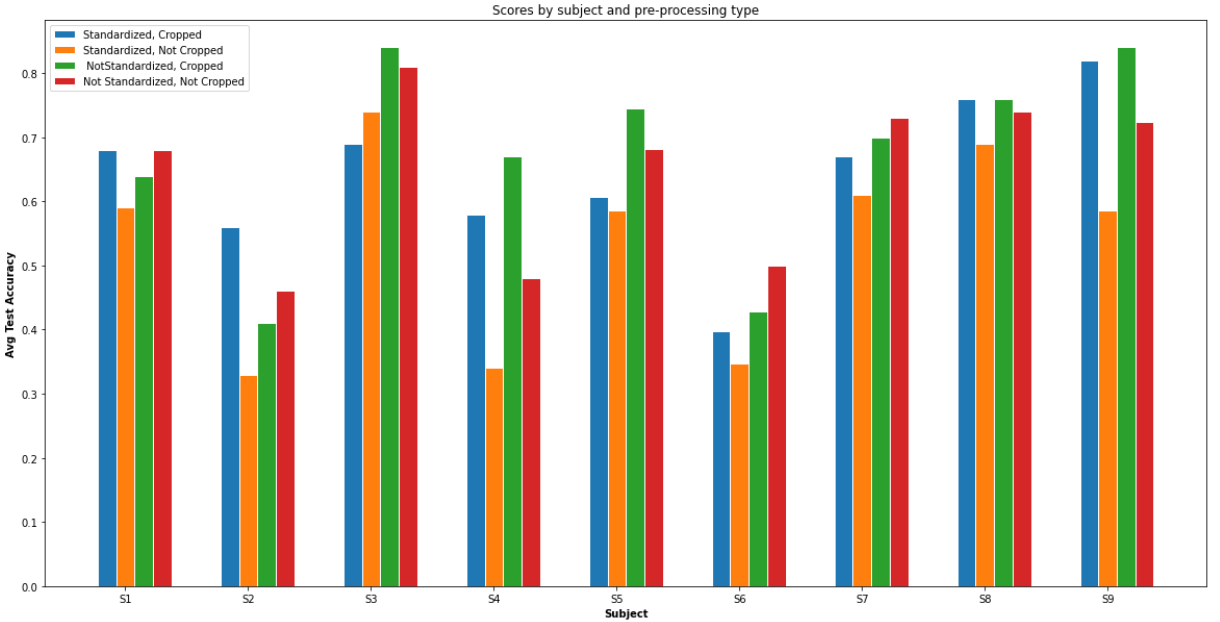
\includegraphics[scale=0.33]{img/subject-scores.png}
    \caption{Classification accuracy for each subject.}
    \label{fig:subj-acc}
\end{figure}

\pagebreak
\subsection{Summary of Results}
% Table with accuracy results across all subjects
\begin{table}[H]
\begin{center}
    \begin{tabular}{|l|c|c|}
        \hline
        Model           & Validation Accuracy & Test Accuracy   \\
        \hline\hline
        Shallow CNN     &                     &                 \\
        SCNN            & 0.704               & 0.654           \\
        SCNN+LSTM       & 0.758               & 0.765           \\
        \hline
    \end{tabular}
\end{center}
\caption{Accuracy results over all subjects in BCI IV dataset 2a.}
\label{tab:acc}
\end{table}

% Table with accuracy results per subject (Shallow CNN)
\begin{table}[H]
\begin{center}
    \begin{tabular}{|c|c|c|}
        \hline
        Subject & Validation Accuracy   & Test Accuracy \\
        \hline\hline
        1       &   &   \\
        2       &   &   \\
        3       &   &   \\
        5       &   &   \\
        6       &   &   \\
        7       &   &   \\
        8       &   &   \\
        9       &   &   \\
        \hline
    \end{tabular}
\end{center}
\caption{Accuracy results for each subject with Shallow CNN model.}
\label{tab:subj}
\end{table}

\subsection{Loss and Accuracy Plots}
Figure \ref{fig:lstm} shows the accuracy and loss over training epochs for the
SCNN+LSTM model. The plot shows how the model begins to overfit the training
data starting around epoch 75. Multiple attempts were made to tune the dropout
parameter to try to reduce overfitting; however, over the limited number of
attemps less overfitting resulted in lower test accuracy.
\begin{figure}[H]
    \centering
    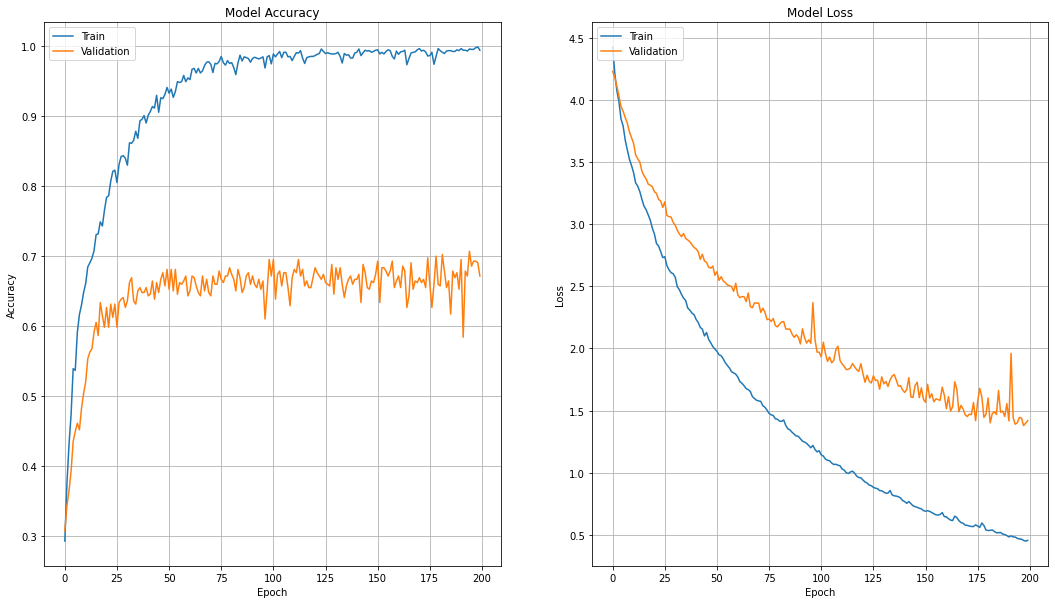
\includegraphics[scale=0.35]{img/scnn.png}
    \caption{Loss and accuracy plots for SCNN}
    \label{fig:lstm}
\end{figure}
\begin{figure}[H]
    \centering
    \includegraphics[scale=0.35]{img/rascnn.png}
    \caption{Loss and accuracy plots for SCNN+LSTM model}
    \label{fig:lstm}
\end{figure}

\pagebreak
\section{Model Architectures}
\subsection{Shallow CNN}
\begin{table}[H]
\begin{center}
    \begin{tabular}{|l|l|l|}
        \hline
        Layer   & Output shape  & Num. of parameters \\
        \hline\hline
        Reshape             & $(N, 22, 500, 1)$     & 0     \\
        Conv2D              & $(N, 22, 476, 40)$    & 1040  \\
        Permute             & $(N, 476, 22, 40)$    & 0     \\
        Reshape             & $(N, 476, 880)$       & 0     \\
        Dense               & $(N, 476, 40)$        & 0     \\
        Activation          & $(N, 476, 40)$        & 35240 \\
        Average pooling 1D  & $(N, 27, 40)$         & 0     \\
        Activation          & $(N, 27, 40)$         & 0     \\
        Flatten             & $(N, 1080)$           & 0     \\
        Dropout             & $(N, 1080)$           & 0     \\
        Dense               & $(N, 4)$              & 4324  \\
        \hline
    \end{tabular}
\end{center}
\caption{Architecture summary for shallow CNN model.}
\label{tab:shallow}
\end{table}

\subsection{SCNN}
\begin{table}[H]
\begin{center}
    \begin{tabular}{|l|l|l|}
        \hline
        Layer   & Output shape  & Num. of parameters \\
        \hline\hline
        Input layer         & $(N, 1000, 22)$       & 0         \\
        Reshape             & $(N, 1000, 22, 1)$    & 0         \\
        Conv2D              & $(N, 1000, 12, 100)$  & 1100      \\
        Conv2D              & $(N, 1000, 1, 100)$   & 120000    \\
        Batch norm          & $(N, 1000, 1, 100)$   & 400       \\
        Spatial dropout 2D  & $(N, 1000, 1, 100)$   & 0         \\
        Conv2D              & $(N, 977, 1, 40)$     & 96000     \\
        Conv2D              & $(N, 954, 1,40)$      & 38400     \\
        Conv2D              & $(N, 931, 1, 40)$     & 38400     \\
        Conv2D              & $(N, 908, 1, 40)$     & 38400     \\
        Batch norm          & $(N, 908, 1, 40)$     & 160       \\
        Average pooling 2D  & $(N, 45, 1, 40)$      & 0         \\
        Spatial dropout 2D  & $(N, 45, 1, 40)$      & 0         \\
        Flatten             & $(N, 1800)$           & 0         \\
        Dense               & $(N, 4)$              & 7204      \\
        \hline
    \end{tabular}
\end{center}
\caption{Architecture summary for SCNN model.}
\label{tab:scnn}
\end{table}

\subsection{SCNN+LSTM}
\begin{table}[H]
\begin{center}
    \begin{tabular}{|l|l|l|}
        \hline
        Layer   & Output shape  & Num. of parameters \\
        \hline\hline
        Input layer         & $(N, 1000, 22)$       & 0         \\
        Reshape             & $(N, 1000, 22, 1)$    & 0         \\
        Conv2D              & $(N, 1000, 12, 100)$  & 1100      \\
        Conv2D              & $(N, 1000, 1, 100)$   & 120000    \\
        Batch norm          & $(N, 1000, 1, 100)$   & 400       \\
        Spatial dropout 2D  & $(N, 1000, 1, 100)$   & 0         \\
        Conv2D              & $(N, 977, 1, 40)$     & 96000     \\
        Conv2D              & $(N, 954, 1,40)$      & 38400     \\
        Conv2D              & $(N, 931, 1, 40)$     & 38400     \\
        Conv2D              & $(N, 908, 1, 40)$     & 38400     \\
        Batch norm          & $(N, 908, 1, 40)$     & 160       \\
        Average pooling 2D  & $(N, 45, 1, 40)$      & 0         \\
        Spatial dropout 2D  & $(N, 45, 1, 40)$      & 0         \\
        Reshape             & $(N, 45, 40)$         & 0         \\
        Birectional LSTM    & $(N, 45, 152)$        & 95080     \\
        Flatten             & $(N, 6840)$           & 0         \\
        Dense               & $(N, 4)$              & 27364     \\
        \hline
    \end{tabular}
\end{center}
\caption{Architecture summary for SCNN+LSTM model.}
\label{tab:lstm}
\end{table}

\pagebreak
\section{Additional Notes}
We performed a series of explorations on the dataset itself, seeking to quantify
any degree of class imbalance, model performance on a per-subject basis, and
model performance on the task of subject classification instead of action
classification. It was found that, while the training set was well-balanced,
the validation and test sets were actually imbalanced: the validation set
contained the largest number of its examples for the ‘Both Feet’ class, whereas
the test set contained the fewest number of its examples in this same class. We
believe that this class imbalance could have caused the dropoff in performance
between validation and test sets for the model described above.

\begin{figure}[H]
    \centering
    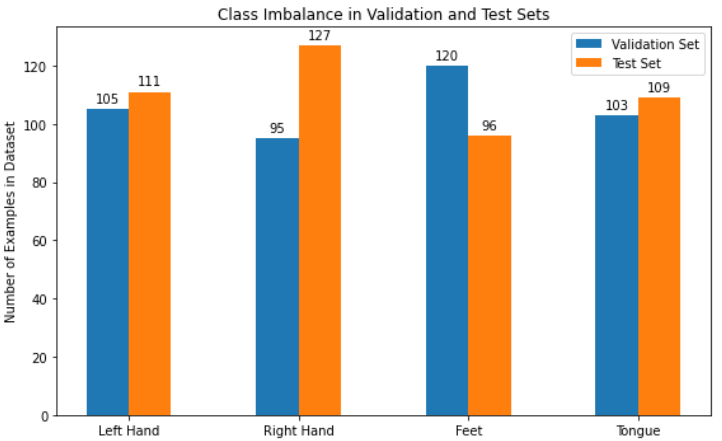
\includegraphics[scale=0.33]{img/imbalance.png}
    \caption{Class imbalance in validation and test sets.}
    \label{fig:imb}
\end{figure}


\end{document}
